\section{Service Models}
\label{sec_service_models}

\IEEEPARstart{Ü}{blicherweise} wird Cloud Computing als Schichtenmodell (vergl. Figure~\ref{fig:serviceModels}) beschrieben, bei dem Schichten durch die Service Modelle charakterisiert werden. Die unterste Schicht bildet die Infrastruktur der Lösung, bestehend aus der zum Betrieb nötigen Hard- und Software. Die darüber liegende Schicht wird als Plattform bezeichnet, sie besteht für gewöhnlich aus einer Sammlung an Werkzeugen und Diensten mit denen das Programmieren und Bereitstellen neuer Cloudanwendungen vereinfacht und beschleunigt wird. Auf diesen beiden Schichten befindet sich die Software Schicht, mit der Endnutzer in Form von bestehenden Webapplikationen interagieren. \cite{rackSpace}

\begin{figure}
	\centering
	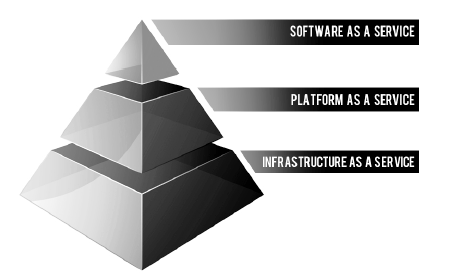
\includegraphics[width=0.95\linewidth]{images/cloudcomputestackimage1}
	\caption{Übersicht Schichten der Servicemodelle}
	\label{fig:serviceModels}
\end{figure}

Auch wenn diese Schichten nicht zusammen genutzt werden müssen, erschließt sich der Zusammenhang jedoch leicht anhand einer Analogie mit der Berliner S-Bahn: Die Schienen bilden die Infrastruktur, die darauf befindlichen Züge stellen die Plattform dar und das S-Bahn Personal, welches die Züge betreibt und so Fahrgäste transportiert dient als Software, welche die ihr zugewiesenen Schienen und Züge nutzt. Im Fall eines Schienenbruchs könnten die Züge auf anderen Strecken zum Einsatz kommen und das Personal könnte auf anderen Verbindungen eingesetzt werden um Fahrgäste zu transportieren.

Dabei gilt es zu beachten, dass die Grenzen zwischen den einzelnen Schichten nicht immer klar gezogen werden können, analog könnte die S-Bahn möglicherweise eine speziell angepasste Antriebstechnik benötigen und so direkt an die Berliner Infrastruktur gekoppelt sein, oder nach der Umstellung auf Draisinen eine der Infrastruktur nähere Betriebsweise eingeführt haben - wodurch der Plattform Charakter in den Hintergrund gerückt werden würde. Als Beispiel einer Infrastruktur die auch gleichzeitig als Plattform fungiert wäre z.B. eine Rolltreppe als Analogie zu betrachten.

Im folgenden Teil der Arbeit werden die verschiedenen Schichten bzw. Service Modelle vorgestellt und auf ebenfalls entstandene Mischformen eingegangen, Tabelle \ref{serviceModelsTable} bildet dabei eine Übersicht über die verschiedenen Modelle.

\begin{figure*}
	\centering
	\begin{tabular}{|l|>{\RaggedRight}p{2cm}|>{\RaggedRight}p{3cm}|>{\RaggedRight}p{3cm}|>{\RaggedRight}p{3cm}|>{\RaggedRight}p{3cm}|}
		\hline
		\rule[-2ex]{0pt}{5.5ex} & \textbf{Paradigmen- wechsel} & \textbf{Merkmale} & \textbf{Vorteile} & \textbf{Nachteile \newline und Risiken} & \textbf{Nicht zu empfehlen bei} \\ 
		\hline
		\rule[-2ex]{0pt}{5.5ex} IaaS & Besitzverhältnis der Infrastruktur & Üblicherweise plattformunabhängig; Infrastruktur-kosten werden geteilt und so reduziert; Service Level Agreements; Nutzungsabhängige Kosten; automatisch skalierend & Kapitalausgaben für Hardware und Betriebspersonal können umgangen werden; ROI Risiken werden verschoben; niedrige Einstiegshürden; optimierte und automatisierte Skalierung & Geschäftsproduktivität und -effizienz hängt stark von den Fähigkeiten des Cloudanbieters ab; potentiell höhere Langzeitkosten; Zentralisierung erfordert neue Sicherheitsmaßnahmen & Größerem Barvermögen als operativem Budget \\ 
		\hline
		\rule[-2ex]{0pt}{5.5ex} PaaS & Lizenzierung & Nutzt Cloud Infrastruktur; eignet sich besonders für agiles Projektmanagement & optimierte Produktveröffentlichung & Zentralisierung erfordert neue Sicherheitsmaßnahmen & - \\ 
		\hline
		\rule[-2ex]{0pt}{5.5ex} SaaS & Besitzverhältnis der Software & Service Level Agreements; Oberfläche meist durch Browser dargestellt; greift auf weitere Cloud Komponenten zu; Kommunikation durch APIs; Zustandslos & Entwicklungskosten können umgangen werden; ROI Risiken werden verschoben; iterative Updates; optimierte Aktualisierung & Zentralisierung der Daten erfordert neue Maßnahmen für die Datensicherheit & - \\ 
		\hline
	\end{tabular}
	\label{serivceModelsTable}
	\caption{Übersicht der Service Arten}
\end{figure*}
 
 
\subsection{Infrastructure as a Service}
Infrastructure as a Service (IaaS) bezeichnet üblicherweise die Bereitstellung von Serverleistung und den dazugehörigen Betriebssystemen, dem Speicherplatz sowie der Netzwerkinfrastruktur. Im Gegensatz zum Kauf der Serverfläche, der Server selber, der Betriebssysteme und deren zugehöriger Software, der zugehörigen Infrastruktur etc. werden hier die benötigten Ressourcen nur nach tatsächlicher Nutzung berechnet.

IaaS stellt für gewöhnlich die Ressourcen ohne Einschränkungen für die Anzahl der Nutzer als Dienst bereit und erlaubt es die bezogene Leistung dynamisch zu skalieren. Mit der Skalierung des genutzten Services wird üblicherweise auch die Berechnungsgrundlage geändert - vergleichbar mit der Berechnung von Strom- oder Gaskosten.

Indem IaaS Anbieter mehr und mehr Konfigurationsunterstützung in Form von Tools und automatisierten Vorgängen bereitstellen, wird die Grenze zur Platform as a Service (PaaS) zunehmend verschoben. Zudem erlauben offene Standards und universell einsetzbare Tools die flexible Kombination von lokal gehosteten Systemen mit denen die durch einen öffentlichen IaaS Anbieter bezogen werden, was als Hybrid Cloud bezeichnet werden kann. \cite{technet}

Aufgrund der weitgehenden Freiheit eines Nutzers bei der Handhabung der genutzten Ressource steht es meist frei Server im Rahmen der Unterstützten Betriebssysteme nach Belieben anzupassen. Im Vergleich zu den noch folgenden Service Modellen Platform- und Software as a Service bietet IaaS damit die höchste Flexibilität und erlaubt z.B. den Einsatz von höchst spezialisierter Software.

Durch die Bereitstellung der bloßen Infrastruktur-Ressourcen beschränkt sich bei diesem Service Modell auch die Service Level Garantie nur auf die Verfügbarkeit der Ressourcen sowie die time to provision einer neuen Einheit. Je nach Ressourcentyp kann dabei jedoch die Garantie für Funktionen die nicht dem Kern des Dienstes entsprechen ausdrücklich verneint werden - so z.B. die Sicherheit der Daten bei einer virtuellen Server Instanz im Vergleich zu der Sicherheit bei einem reinen Cloud Speicheranbieter. Die Verantwortung zur Wahrung solcher Interessen obliegt hier zum größten Teil dem Nutzer. Zudem bedeutet die Nutzung einer nicht eigenen Infrastruktur in der Regel auch eine zunehmende Latenz der errechneten Ergebnisse, sowie einen erhöhten Zeitaufwand beim laden der zu verarbeitenden Daten.

Sinnvoll erscheint die Nutzung von IaaS daher vor allem wenn die dynamische Skalierung der Ressourcen nötig ist, d.h. wenn kurzzeitig eine verstärkte Nachfrage auftritt oder ein plötzlich auftretendes Wachstum der Nutzerbasis eine solche Skalierung verlangt. Zudem ist IaaS für Unternehmen interessant deren Kapitalressourcen nicht ausreichen um die nötige Menge an Hardware zu beschaffen um die für die Geschäftsidee nötigen Systeme zu betreiben. Überdies kann IaaS häufig auch bei Testprojekten oder nur ausgewählten Geschäftsgebieten machen, sodass der Betrieb eines Unternehmens allein auf Basis von IaaS nicht nötig ist.

Von IaaS als Lösung ist jedoch abzuraten wenn die zuvor erwähnten Nachteile überwiegen, d.h. eine sehr große Datensicherheit nötig ist oder die Gesetzeslage es verbietet Daten außerhalb der eigenen Unternehmensgrenzen zu lagern. Auch wenn es sich vor allem um die hochperformante Verarbeitung von großen Datenmengen handelt, die nicht direkt für die auf dem IaaS laufende Anwendung zugänglich ist, ist der zeitliche Mehraufwand beim Datentransfer zu bedenken und eine dedizierte Lösung eventuell besser geeignet. \cite{technet} \cite{rackSpace} \cite{ibm2011}

\subsection{Platform as a Service}
Platform as a Service (PaaS) erweitert die Möglichkeiten des IaaS um Entwicklungsspezifische Punkte, sodass ein PaaS Anbieter für gewöhnlich vorkonfigurierte Entwicklungs- und Laufzeitumgebungen anbietet, die nach Bedarf in der Leistung und Größe skaliert werden können. Wie bei IaaS ist es nicht nötig die Hardware auf der die Software laufen soll zu kaufen, diese wird als Teil des Services gestellt. PaaS Anbieter müssen dank der Möglichkeiten von IaaS nicht einmal selber Infrastruktur besitzen, sondern können sich auf die Optimierung der für ihr PaaS Geschäft nötigen Software konzentrieren. 

Die Leistung einer PaaS besteht dabei jedoch nicht in der Bereitstellung der Software als solches, sondern der Plattform die durch die Software des Anbieters betrieben wird. Üblicherweise bietet ein PaaS Unterstützung für die Entwicklung, das Testen, die Veröffentlichung, den Betrieb sowie die Wartung von Anwendungen in der selben Entwicklungsumgebung. Der Zugriff auf die Umgebung ist dabei multi-tenant fähig, sodass speziell agile Entwicklungsmethoden mit verteilten Entwicklerteams unterstützt werden. 

Die Entwicklungsunterstützung kann dabei in Form von vordefinierten UI Elementen, vorkonfiguriertem Load-Balancing und Skalierungsmaßnahmen bis hin zur Integration mit anderen Webdiensten, Datenbank und Hardware erfolgen. Aufgrund der zunehmenden Verbreitung von Standards in der Entwicklung ist es zudem leicht möglich diese vordefinierten Funktionen zu erweitern. 

Meistens unterscheiden sich die verschiedenen Plattformen im Ausmaß der Vorarbeit bzw. der Konfigurierbarkeit, diese kann von der Entwicklungsumgebungen reichen, bei denen allein die Laufzeitumgebung sowie die Kontrolle über die Leistungsfähigkeit der angeforderten Instanz gegeben wird bis hin zu vorkonfigurierten, komplexen UI Elementen zur Verarbeitung von bereitgestellten Daten, mit denen ohne Programmieraufwand eine Anwendung entwickelt werden kann.

Aufgrund des Fokus' auf die Entwicklungsunterstützung bietet PaaS auch hier den größten Vorteil, da komplexe IT Anwendungen häufig von komplexen Entwicklungsstrukturen begleitet werden. Damit einher gehend ist die Nutzung von PaaS ebenfalls für Entwicklungen mit automatisierten Tests und häufigen Iterationen zu empfehlen, da der hohe Automatisierungsgrad eine ständige Neuinstallation stark vereinfacht und somit die dabei auftretenden Probleme von Beginn an behandelt werden können.

Allerdings gilt es bei PaaS den Einsatzzweck auf die Nutzbarkeit mit einem PaaS zu überprüfen sowie bei der vom PaaS verwandten Technologie darauf zu achten ob man einem Vendor lock-in entgehen könnte. Wie auch bei IaaS ist auch hier die Performancebetrachtung wichtig, da die standardisierten Umgebungen wenig Spielraum zulassen, spezielle Betriebssystemfunktionen oder Fremdsoftware zu nutzen bzw. anzupassen, im Gegensatz zu IaaS gilt diese Limitierung auch beim Betrieb einer eigenen PaaS Umgebung. \cite{technet} \cite{rackSpace} \cite{ibm2011}

\subsection{Software as a Service}
Software as a Service (SaaS) bildet die oberste Schicht in der schichtweisen Betrachtung des Cloud Computing und wird so auch häufig durch die Nutzung einer der beiden darunter liegenden Schichten realisiert. Im Vergleich zu den vorherigen Modellen ist die so angebotene Software von den darunter befindlichen Strukturen abstrahiert und für Endnutzer zugänglich. Software die als SaaS angeboten wird, kann vom Nutzer über ein Netzwerk genutzt werden und verlangt so keine Installation. Diese Auslieferungsmethode bringt zudem den Vorteil, dass Nutzer sich nicht mehr um die Wartung der Software kümmern müssen und bei der Entwicklung von einer deutlich geringeren Versionsfragmentierung ausgegangen werden kann. Wie auch bei den vorangegangenen Schichten wird die SaaS Schicht durch APIs erweiterbar gehalten und nutzt für gewöhnlich fremde APIs um realisiert zu werden.

Vor allem durch den hohen Grad an Standardisierung der Software bietet sich die Nutzung von SaaS für grundlegende Softwaresysteme an, die nicht zum Kernbereich des jeweiligen Unternehmens zählen, email- sowie CRM-Systeme stellen hier ein gängiges Beispiel für den SaaS Einsatz dar. Derartige Systeme sind typischerweise für den laufenden Betrieb eines Unternehmens wichtig, bieten jedoch selten einen großen Wettbewerbsvorteil bei eigenen Anpassungen. Durch die Vereinbarung von Service Level Agreements ist es vor allem möglich eine gute Erreichbarkeit der Lösung zu gewährleisten - üblicherweise liegt die zugesicherte Erreichbarkeit der Systeme bei 99\% und höher. Auch hier werden derartige Dienste entsprechend der Nutzungsdauer bezahlt.

Die leichten Skalierungsmöglichkeiten der einer SaaS Lösung zugrunde liegenden Cloud Infrastruktur erweist sich als weiterer Indikator auf den Einsatz einer solchen Lösung zu setzen. Ist es zu erwarten, dass die Software nur über kurze Zeiträume unter hoher Last stehen wird, wie z.B. bei Verkaufssystemen vor Weihnachten oder zu Beginn eines neuen Jahres. Auch wenn die Nutzung der Software nur für einen begrenzten Zeitraum benötigt wird, bietet sich die Verwendung von SaaS an. Ebenso kann das über ein Netzwerk erfolgende Angebot der Software ausgenutzt werden, da Anwendungen mit einem hohen Grad an Interaktion mit anderen Systemen leichter mit diesen sowie weiteren Diensten kommunizieren können. Mit Blick auf die zunehmende Verbreitung der mobilen Internet Nutzung sowie der verbreiteten Unterstützung verschiedener Anzeigegrößen im SaaS Umfeld, ist der Einsatz einer SaaS Lösung auch von Interesse wenn ein möglichst nahtloser Übergang zwischen verschiedenen Gerätetypen gewährleistet werden soll, da die SaaS-Anwendung die selbe bleibt und so z.B. keine Brüche im Datenbestand auftreten. Nicht zuletzt ist eine SaaS Lösung zu empfehlen wenn die Versionsfragmentierung minimal gehalten werden soll.

Im Gegenzug bietet sich eine SaaS Lösung nicht an wenn die benötigte Funktion bereits durch eine existierende on-premise abgedeckt wird, d.h. bestehende Systeme durch eine SaaS Einführung nicht weiter genutzt werden würden. Ebenso stellt, wie auch bei der IaaS, die Gesetzgebung oder die Firmengrundsätze eine Entscheidungsgrundlage dar, ist vor allem bei einer öffentlichen SaaS Lösung nicht auszuschließen, dass Daten das Land oder das Firmennetzwerk verlassen. Und ebenfalls wie bei der IaaS zutreffend ist auch bei SaaS die nötige Verarbeitungsgeschwindigkeit entscheidend, die sofortige Verarbeitung anfallender Echtzeitdaten kann bei SaaS nicht immer gewährleistet sein und so eine on-premise Lösung erstrebenswerter machen. \cite{technet} \cite{rackSpace} \cite{ibm2011}

\subsection{Everything as a Service}
Neben den hier aufgeführten Modellen wird das Servicemodell auch in anderen Formen in Verbindung zum Cloud Computing gebracht, so gibt es die Möglichkeit Business Process as a Service zu nutzen um z.B. weitere Teile des Tagesgeschäfts automatisieren zu können, zudem werden auch die eventuell nötigen Schritte zur Skalierung oder zum Start einer Cloudlösung angeboten und als Cloudsetup as a Service vertrieben. Der Computing Aspekt ist dabei weit weniger im Vordergrund als bei den vorangegangenen Modellen. Überdies gibt es Spezialisierungen der Modelle, sodass der Betrieb angepasster Datenbanken als Database as a Service betrieben wird oder Plattformen die mit minimalem Aufwand zur vollständigen Software as a Service aufgebaut werden können, wofür Wordpress as a Service beispielhaft ist.

\section{Private vs. Public}
\label{sec_privacy_models}

\IEEEPARstart{U}{nabhängig} von der Serviceform erfolgt die Einteilung zudem nach der Art der Bereitstellung eines Clouddienstes. Dabei richtet sich die Unterscheidung nach dem Eigentumsverhältnis der zugrundeliegenden Systeme und dem damit verbundenen Grad an Anpassbarkeit. Die Anpassbarkeit bezieht sich dabei sowohl auf die Architektur als auch auf die des jeweiligen Dienstes. 

Aus diesen Unterscheidungen ergeben sich ferner weitere Charakteristiken der einzelnen Bereitstellungsmodelle - dargestellt in Tabelle \ref{deploymentTypesTable}. Abhängig von der Bereitstellung variieren die Kosten, die Kontrollmöglichkeit und die Skalierbarkeit.

\begin{figure*}
	\begin{tabular}{|>{\RaggedRight}p{3cm}|>{\RaggedRight}p{1.6cm}|>{\RaggedRight}p{2.2cm}|>{\RaggedRight}p{2.5cm}|>{\RaggedRight}p{2.7cm}|>{\RaggedRight}p{3cm}|}
		\hline
		\rule[-2ex]{0pt}{5.5ex} \textbf{Art der \newline  Bereitstellung} & \textbf{Hosting} & \textbf{Geteilt oder Dediziert} & \textbf{Kontrolle über Architektur} & \textbf{Skalierbarkeit} & \textbf{Art der Investition} \\ 
		\hline
		\rule[-2ex]{0pt}{5.5ex} Shared Public & Extern & geteilt & Cloudanbieter oder Markt & minimale Einschränkungen & Nutzungsabhängig \\ 
		\hline
		\rule[-2ex]{0pt}{5.5ex} Dedicated Public & Extern & (Teilweise) dediziert & Cloudanbieter oder Markt & Vertragsabhängig & Nutzungsabhängig \\ 
		\hline
		\rule[-2ex]{0pt}{5.5ex} Self Hosted Private & Intern & Dediziert & Voll & Investitionsabhängig & Cloud-Aufbau, ROI durch Serviceangebot \\ 
		\hline
		\rule[-2ex]{0pt}{5.5ex} Hosted Private & Extern & Dediziert & Voll & Vertrags- oder Investitionsabhängig & Vertragsabhängig, möglicherweise mit Auswirkung auf Barvermögen \\ 
		\hline \rule[-2ex]{0pt}{5.5ex} Private Appliance & Intern & Dediziert & Cloudanbieter & Angebotsabhängig & Vertragsabhängig, möglicherweise mit Auswirkung auf Barvermögen \\ 
		\hline 
	\end{tabular}
	\centering
	\caption{Deployment Arten Übersicht}
	\label{deploymentTypesTable}
\end{figure*}

\subsection{Public Cloud}
Anbieter von IT Ressourcen als SaaS, PaaS und speziell als IaaS müssen die Rechenleistung in Form von Rechenzentren bereitstellen, um die Verfügbarkeit dieser Ressourcen über weite Strecken zu gewährleisten, erfolgt dies in der Regel über Orts- und Ländergrenzen hinweg. Im Fall einer public Cloud befindet sich die zugrundeliegende Schicht im Eigentum des jeweiligen Cloud Anbieters.

Diese Ressourcen werden mehreren Kunden zur Verfügung gestellt, was zu einer Kostenreduktion für den einzelnen Nutzer führt und die vorhandenen Kapazitäten besser ausnutzt - z.b. indem die nicht benötigte Leistung eines Kunden sinnvoll mit dem Abfangen eines hohen Leistungsbedarfs eines anderen Kunden kombiniert werden kann.
Im Gegenzug bedeutet diese Ressourcenteilung jedoch z.B. auch die gemeinsame Nutzung von Speicher bzw. die geringere Kontrolle über die eingesetzte Software und die so verarbeiteten Daten.

Die vorgestellten Service Modelle (IaaS, PaaS und SaaS) sind alle sowohl als private als auch als public Lösung zu finden.

Auch das Angebot der Public Cloud bietet weitere Unterscheidungsmöglichkeiten in Bezug auf die Hosting Form.

\subsubsection{Shared Public Cloud}
Wird der Service auf einer mit mehreren Benutzern geteilten Schicht betrieben, deren Architektur, Absicherung und Verwaltung durch den Anbieter erfolgt, wird von einer Shared Public Cloud gesprochen. Auch die Anpassbarkeit wird hier durch den Anbieter vorgegeben. Durch diese Bedingungen ist es möglich besonders günstige Kosten für den Betrieb zu veranschlagen und den Umfang der Serviceleistung nach Bedarf zu skalieren. 

\subsubsection{Dedicated Public Cloud/ Virtual Private Cloud}
Das direkte Gegenstück zur Shared Public Cloud bildet die Dedicated Public Cloud, bei der ein Teil der Ressourcen der Shared Public Cloud einem Kunden dediziert zur Verfügung gestellt werden. Durch den Ausschluss weiterer Nutzer der selben Infrastruktur bietet sich häufig eine bessere Leistungsfähigkeit als bei der Shared Public Cloud, ebenso können meist mehr Sicherheitsmaßnahmen getroffen werden und anderweitige Anpassungen des Dienstes vorgenommen werden. Auch wenn es sich um dedizierte Systeme handelt, erfolgt das Hosting der Dienste auf Systemen im Besitz des Anbieters.

\subsection{Private Cloud}
Die IT Ressourcen werden bei einer Private Cloud exklusiv für einen Kunden bereitgestellt. Damit können Anforderungen an Sicherheit, Privatsphäre im hohen Maß erfüllt werden und das Vertrauen in die Cloud Lösung erhöht werden. Dazu bietet eine derartige Lösung die Möglichkeit innerhalb des zur Verfügung stehenden Vorrats an Ressourcen nach Bedarf zu skalieren und diese Ressourcen so bestmöglich zu nutzen.

Die Verwendung einer privaten Cloud Lösung bietet sich vor allem an, wenn das Gesetzes- oder Unternehmensumfeld strenge Vorgaben an den Betrieb der IT stellt oder das Vertrauen in einen passenden Cloudanbieter nicht ausreicht um die nötige Lösung in dessen Public Cloud zu hosten. 

Wie auch bei der Public Cloud kann die Private Cloud anhand der Hosting Form unterschieden werden.

\subsubsection{Self-Hosted Private Cloud}
Die Self-Hosted Private Cloud stellt auf Basis der bestehenden Systeme und Services eine im Rahmen dieser skalierbare Cloud Umgebung. Dadurch behält man die volle Kontrolle über die Systeme, kann die Architektur nach Belieben anpassen und die Auslastung der Systeme maximieren.

\subsubsection{Hosted Private Cloud}
Im Vergleich zur Dedicated Public Cloud/ Virtual Private Cloud, ist die Hosted Private Cloud zwar ebenfalls im Data-Center eines Cloudanbieters angesiedelt und wird mittels der Dienste dieses Anbieters betrieben, allerdings können die dazu nötigen Systeme vom Kunden angepasst werden und werden durch den Kunden dediziert gemietet. Durch diese Konstellation lässt sich der Vorteil einer in einem Data-Center befindlichen Lösung mit der Kontrolle wie bei einer Self-Hosted Private Cloud kombinieren.

\subsubsection{Private Cloud Appliance}
Bei einer Private Cloud Appliance wird eine von einem Cloudanbieter entworfene und angepasste Cloudumgebung beim Kunden installiert und durch diesen oder den Cloudanbieter selbst gewartet. Dadurch ist es möglich die Interoperabilität der Dienste des Cloudanbieters nutzen zu können ohne die Sicherheit oder die Kontrolle über die Daten einzuschränken, allerdings ist die Skalierung meist nur im Rahmen der vorhandenen Umgebung möglich.

\subsection{Hybrid Cloud}
Neben der Unterscheidung in Private- und Public Cloud ergibt sich auch ein Raum für Mischformen, bei denen verschiedene Cloud Infrastrukturformen miteinander kombiniert werden. Die Komposition erfolgt dabei so, dass die Teilbestandteile eigenständig funktionieren, bei Bedarf jedoch zwischen den Bestandteilen ausgetauscht werden kann um z.B. Lastspitzen abzufangen oder um Teilberechnungen auf einem angepassten Dienst durchzuführen. Als Hybrid Cloud werden auch Systeme bezeichnet, die verschiedene Dienste der gleichen Infrastrukturform komponieren wie z.B. mehrere Public Cloud Dienste.

Besonders bietet sich diese Form an, wenn datenschutzkritische Prozesse gesondert in einer Private Cloud und datenschutzunkritische Prozesse in einer Public Cloud bearbeitet werden können, da so die Einspar- sowie Skalierungsmöglichkeiten der Public Cloud genutzt werden und gleichzeitig die Datenexposition verhindert werden kann. Die Unterteilung von Geschäftsprozessen in diese Kategorien stellt dabei jedoch keine geringe Hürde dar. \cite{technet}